\section*{Introduction} % Pas de numérotation
\addcontentsline{toc}{section}{Introduction} % Ajout dans la table des matières

\subsection*{Objectif}
Ce projet a pour objectif de réaliser une modélisation 
d'un résolveur de sudoku en langage Java.

\subsection*{L'origine du sudoku}
Le sudoku a été inventé en 1979 par Howard Garns, un pigiste spécialisé dans les
puzzles, et publié cette même année pour la première fois dans Dell Magazines sous le
nom de Number Place. Après avoir été introduit au Japon, le nom devient Sudoku. En
2004, Le Times publie une première grille puis les autres journaux suivent. Depuis, le
phénomène a fait le tour du monde et est arrivé en France. Inspiré du carré latin de Leon-
hardt Euler, le but du jeu est que chaque ligne, colonne et région de 3x3 cases contienne
chaque chiffre de 1 à 9 une seule fois.

Actuellement, il existe de nombreuses variantes pour le sudoku allant 
de la plus simple à la plus complexe. Comme exemple, nous avons : changer 
la taille de la grille et ne plus prendre systématiquement 3x3 cases mais 2x2 cases 
(idéal pour apprendre, se familiariser lorsque c'est la première fois que l'on joue), 
ou encore 10x10 cases si on aime les défis. Parmi ces variantes nous trouverons également
la possibilité de remplacer les chiffres par des symboles ainsi, à la place de 
compter en base 10, nous pourrions compter en base 16, en hexadécimal, 
de 0 à F (pour des régions 4x4).

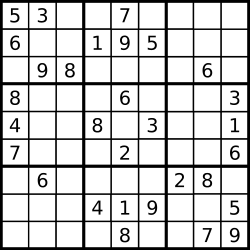
\includegraphics [width=60mm]{images/sudokuOriginale.png} \\[0.5cm]